\section{Задача поиска ближайшего соседа}
\begin{center}
    Конспект составил: \textit{Азим Мурадов}
\end{center}

\subsection{Постановка задачи}

Дано множество точек $S$ ($|S| \geq 2$), расположенных в метрическом пространстве. Среди них выбрана точка $x$.
Нужно найти \textbf{одного из ближайших соседей} $x'$ для точки $x$, согласно некоторой заданной функции близости, определяющей это метрическое пространство.

\begin{figure}[H]
    \centering
    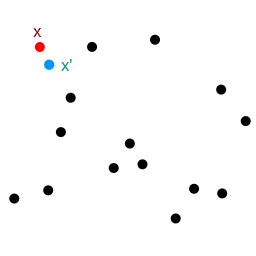
\includegraphics[width=0.6\linewidth]{points.png}
    \caption{Иллюстрация задачи}
\end{figure}

В этой лекции задача будет демонстрироваться для двумерного Евклидова пространства в Декартовой системе координат.

\subsection{Идеи решения}

\subsubsection*{Диаграмма Вороного}

\textbf{Диаграмма Вороного} конечного множества точек $S$ на плоскости представляет собой такое разбиение плоскости, при котором каждая область этого разбиения образует множество точек, более близких к одному из элементов множества $S$, чем к любому другому элементу множества.

\begin{figure}[H]
    \centering
    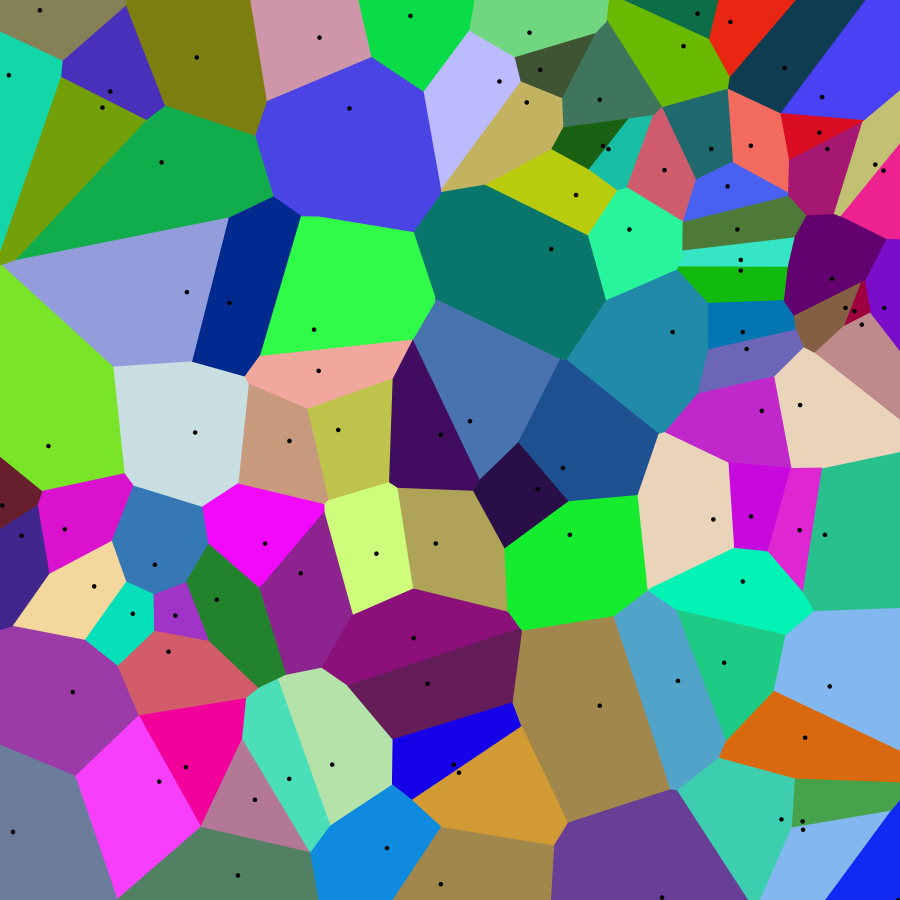
\includegraphics[width=1\linewidth]{voronoi-diagram.png}
    \caption{Диаграмма Вороного}
\end{figure}

\subsubsection*{Триангуляция Делоне}

\textbf{Триангуляция Делоне} — триангуляция для заданного множества точек $S$ на плоскости, при которой для любого треугольника все точки из $S$, за исключением точек, являющихся его вершинами, лежат вне окружности, описанной вокруг треугольника.

\begin{figure}[H]
    \centering
    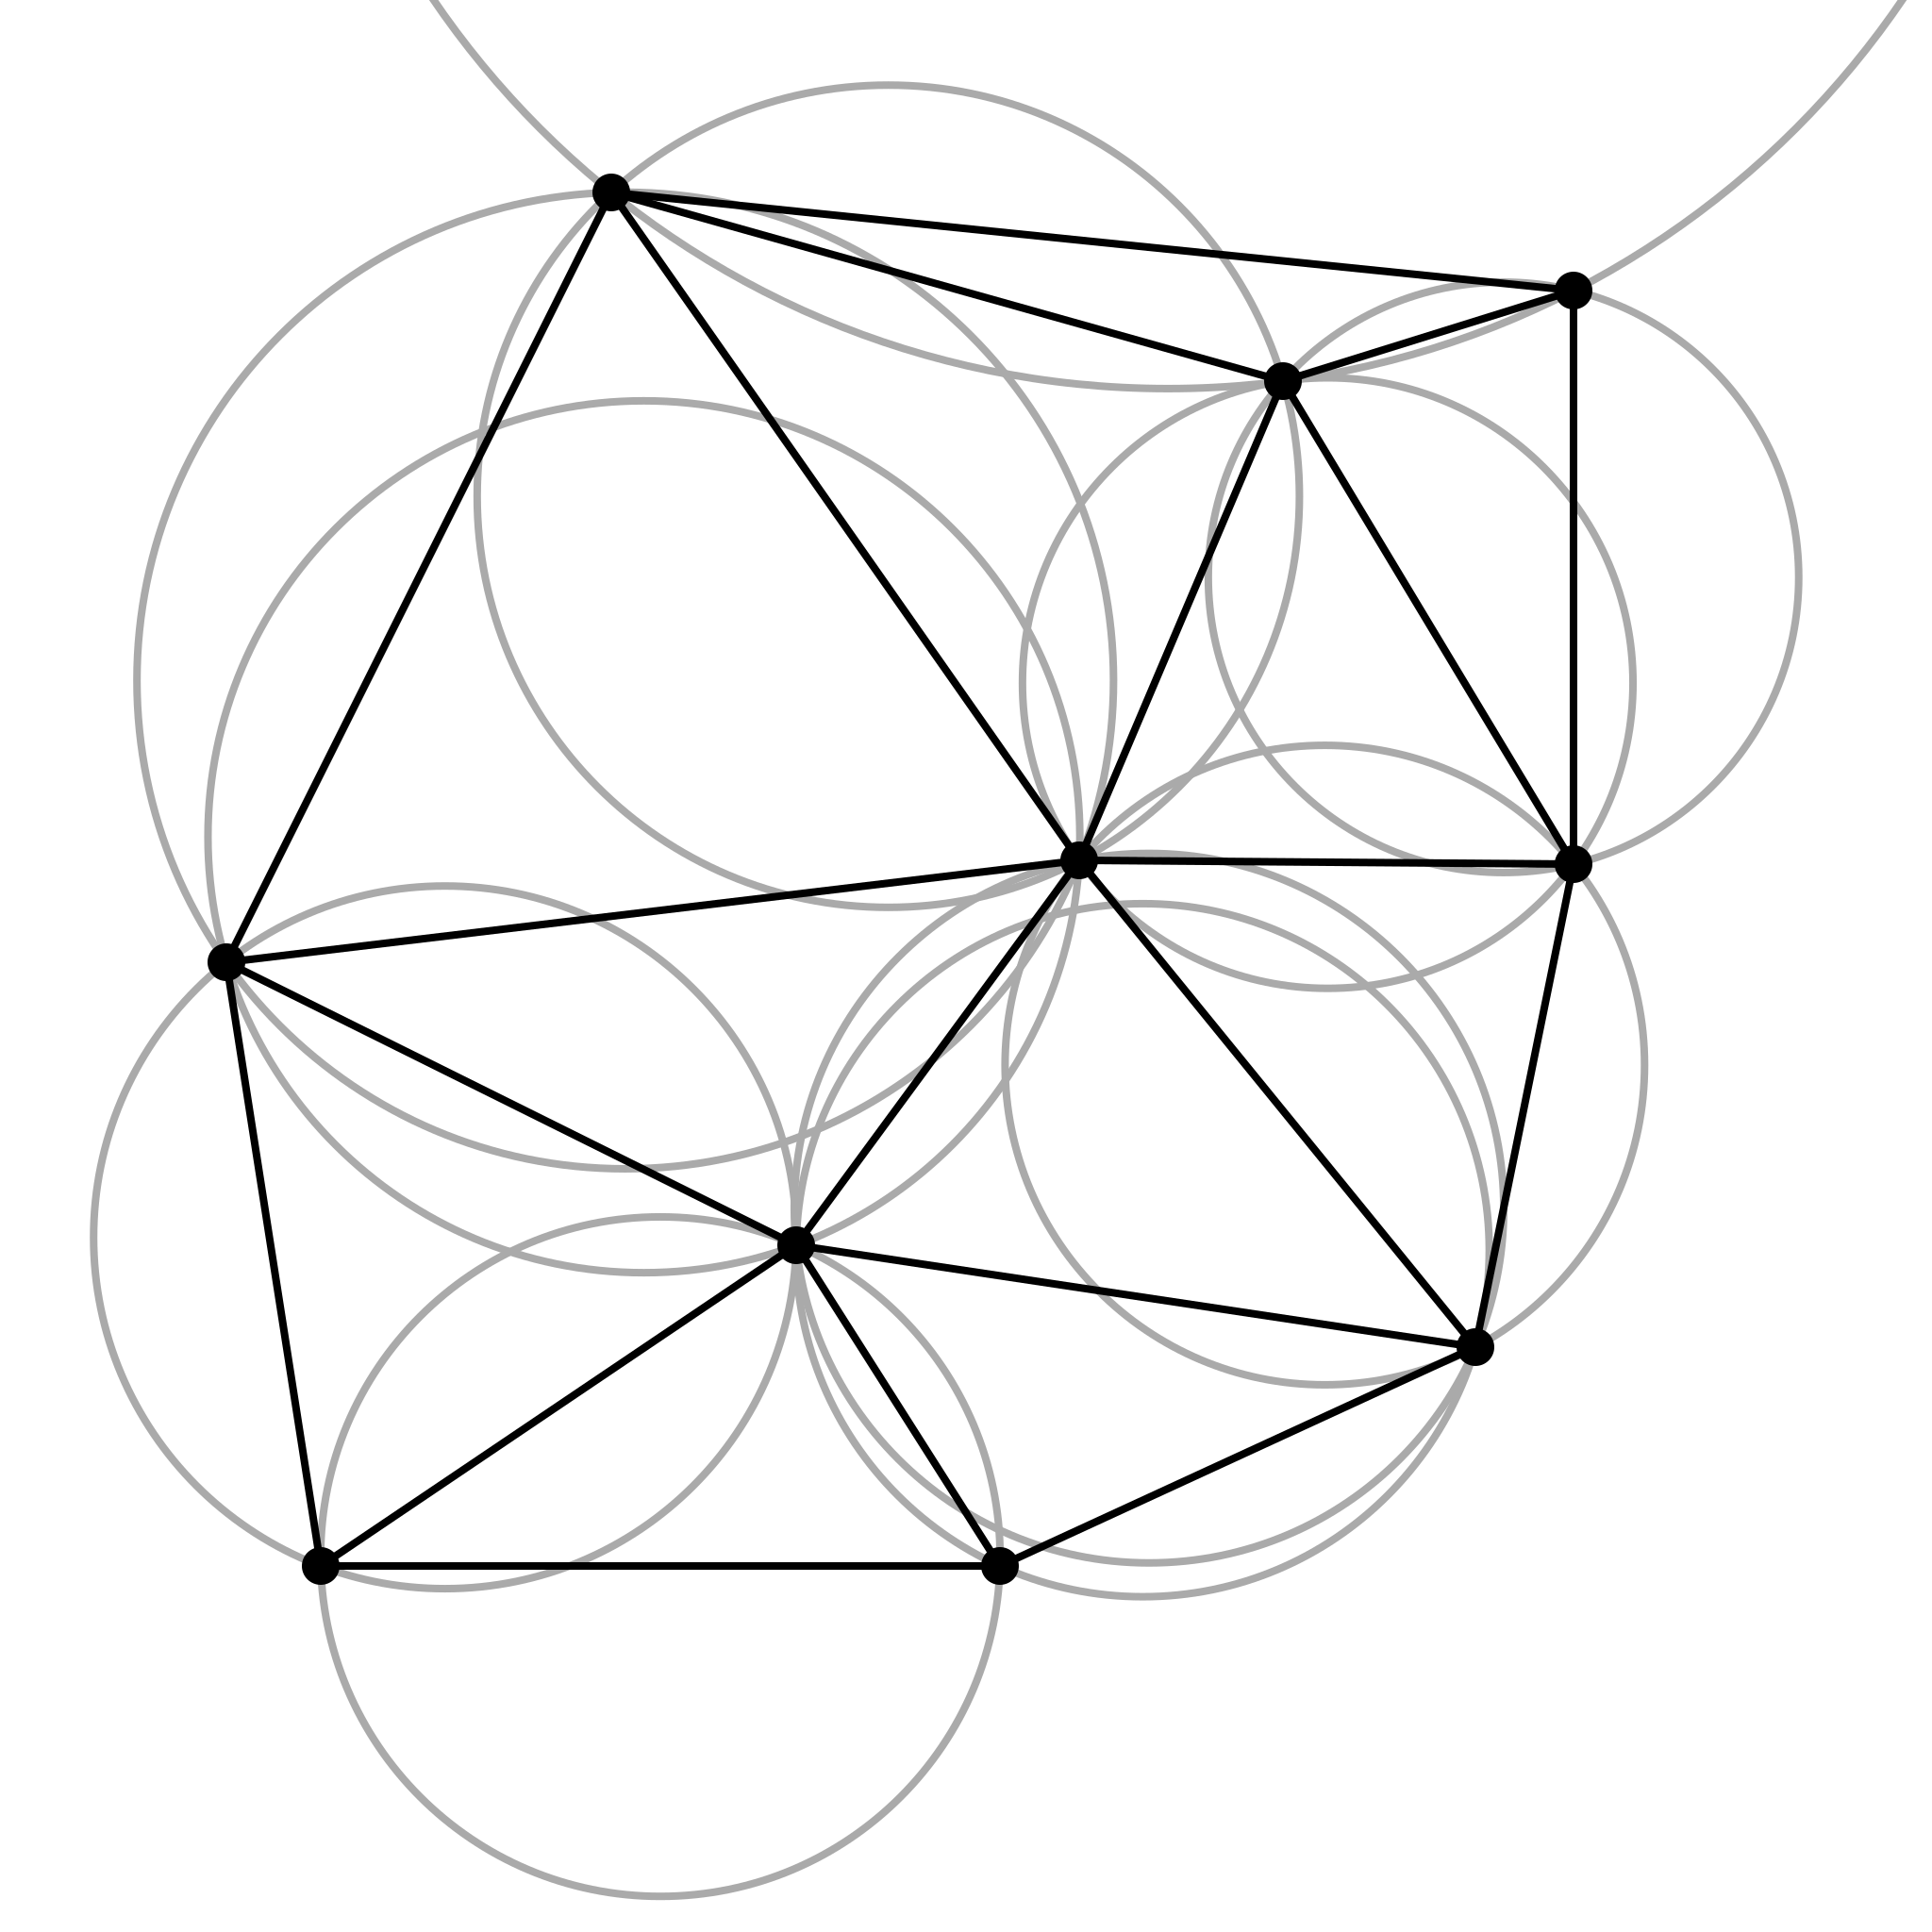
\includegraphics[width=0.75\linewidth]{delaunay-circumcircles-vectorial.png}
    \caption{Триангуляция Делоне}
\end{figure}

\newpage

\subsubsection*{Связь диаграммы Вороного с триангуляцией Делоне}

Диаграмма Вороного имеет взаимно-однозначное соответствие с триангуляцией Делоне. Если соединить рёбрами точки, области Вороного которых граничат друг с другом, полученный граф будет являться триангуляцией Делоне.

\begin{figure}[H]
    \begin{center}
        \begin{minipage}[h]{0.45\linewidth}
            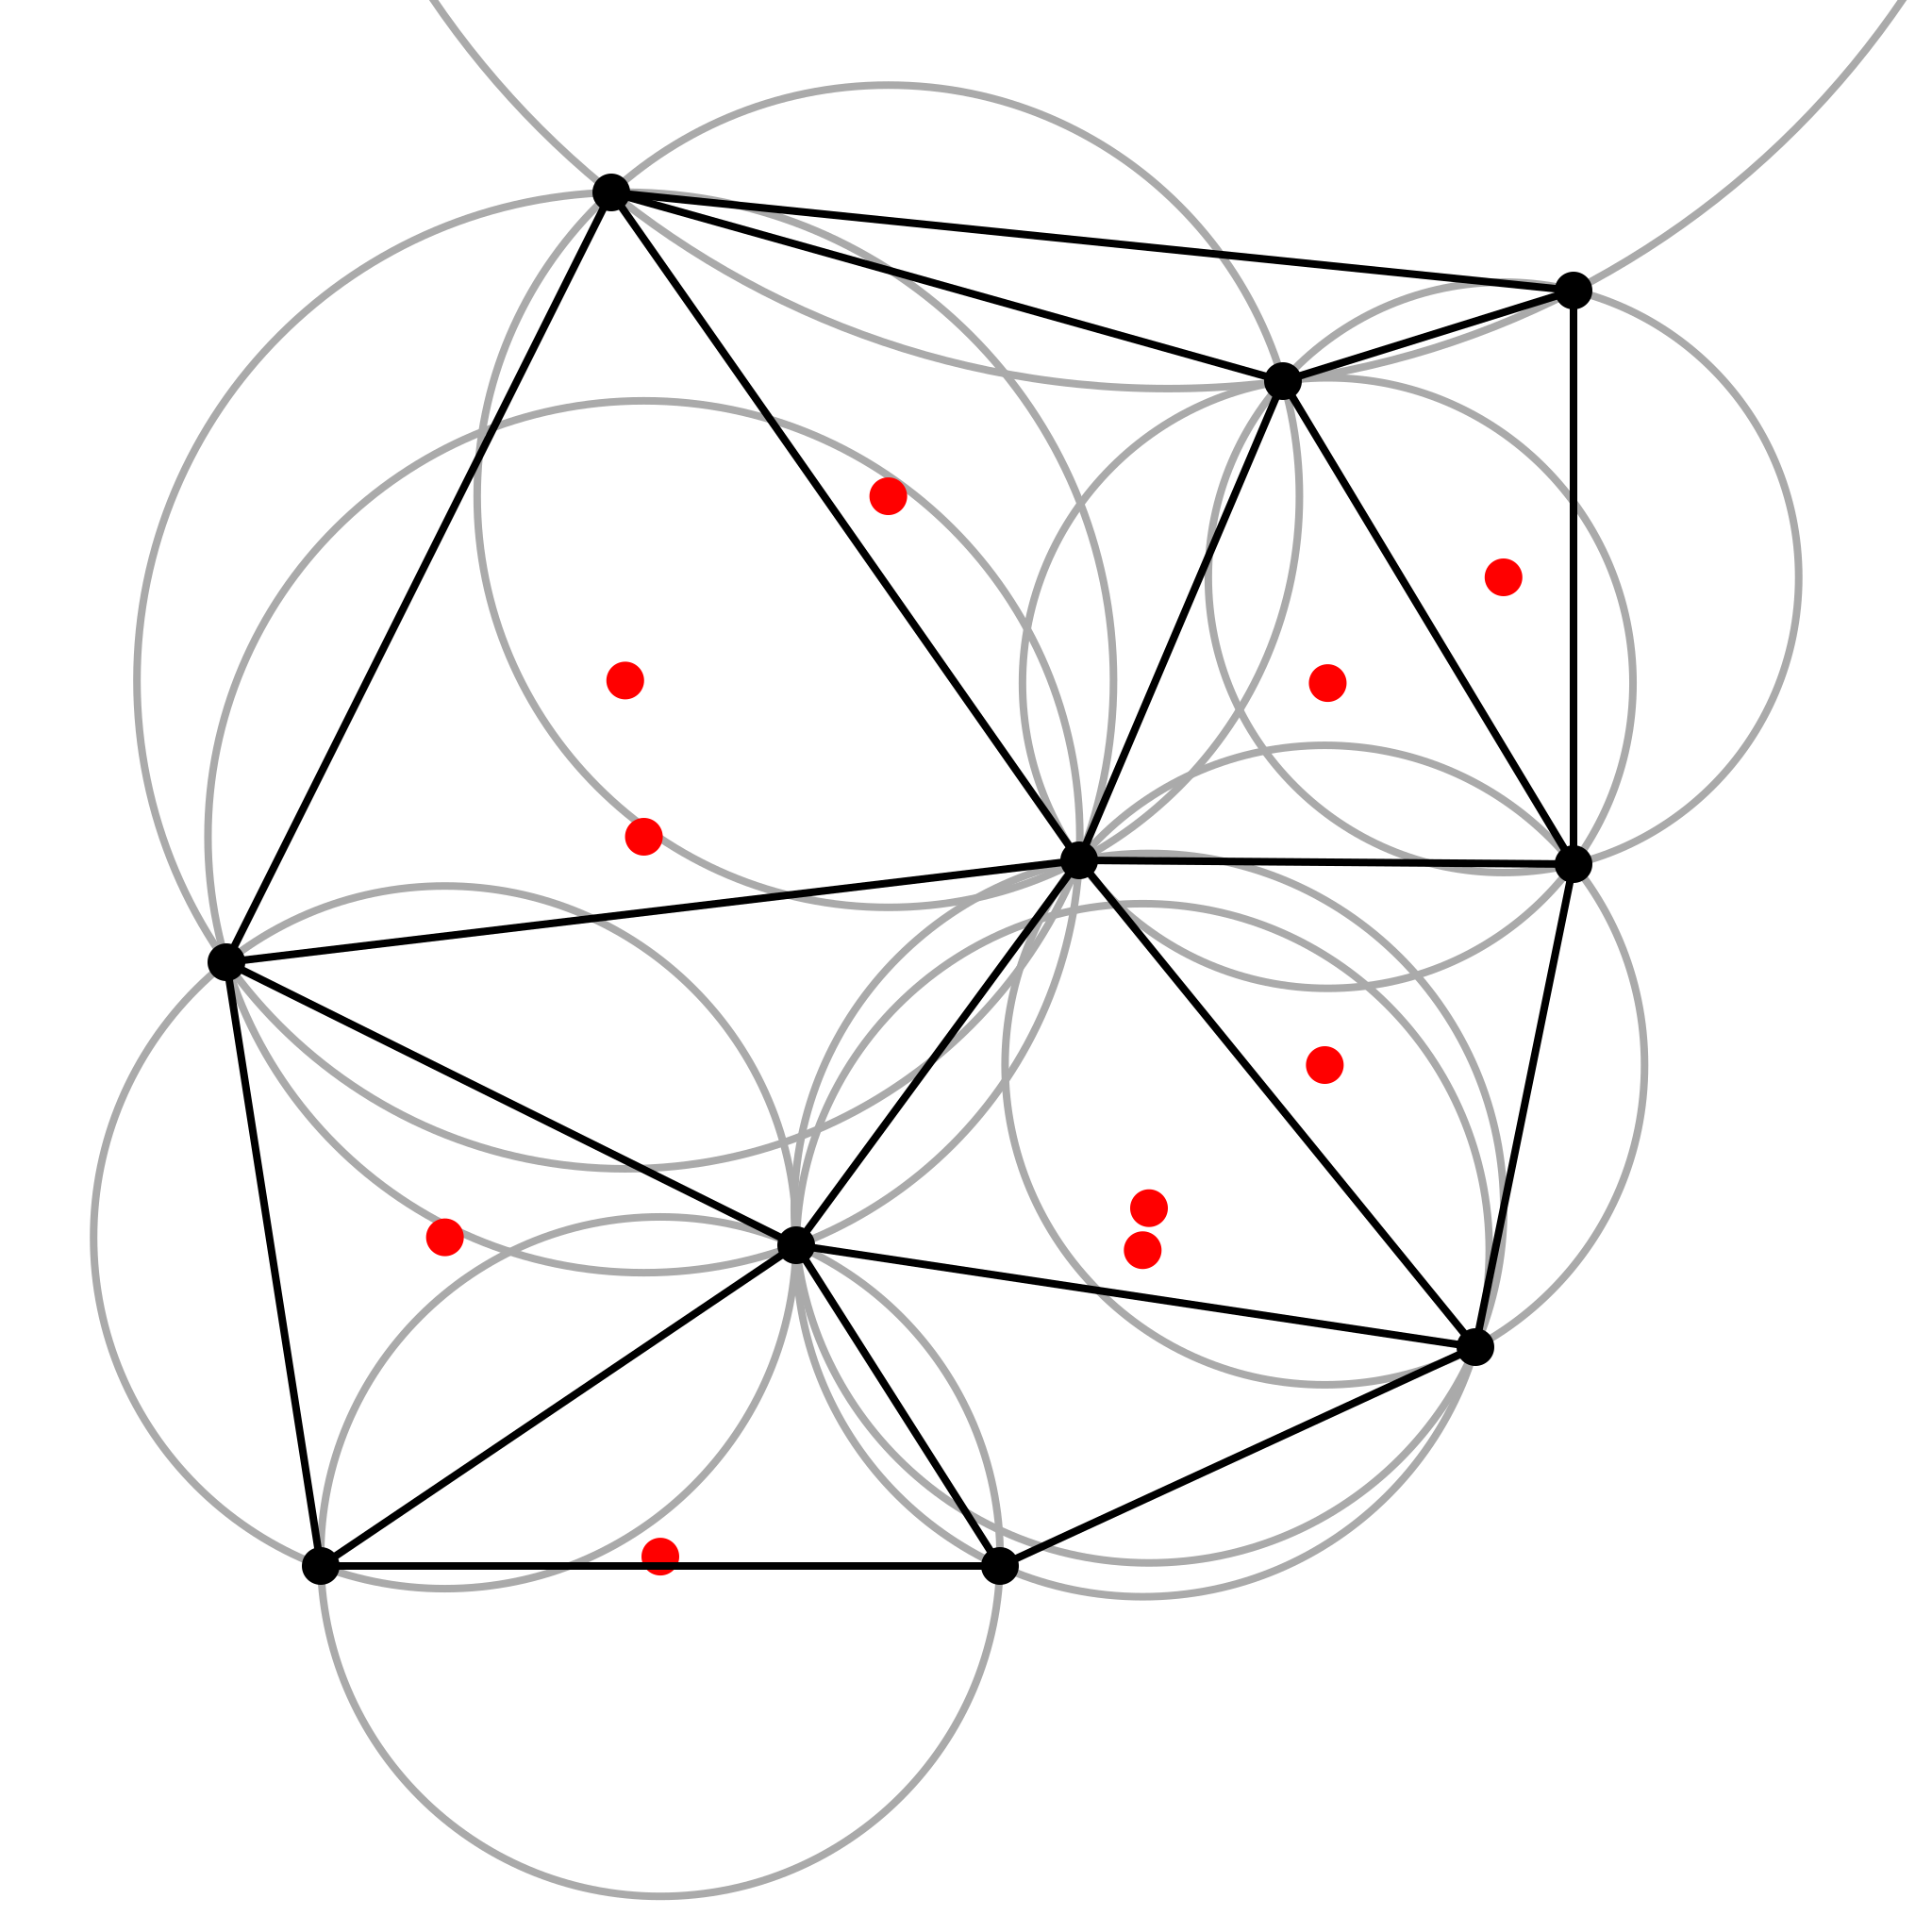
\includegraphics[width=1\linewidth]{delaunay-circumcircles-centers.png}
            \caption{Триангуляция Делоне со всеми описанными окружностями и их центрами (красными).}
        \end{minipage}
        \hfill
        \begin{minipage}[h]{0.45\linewidth}
            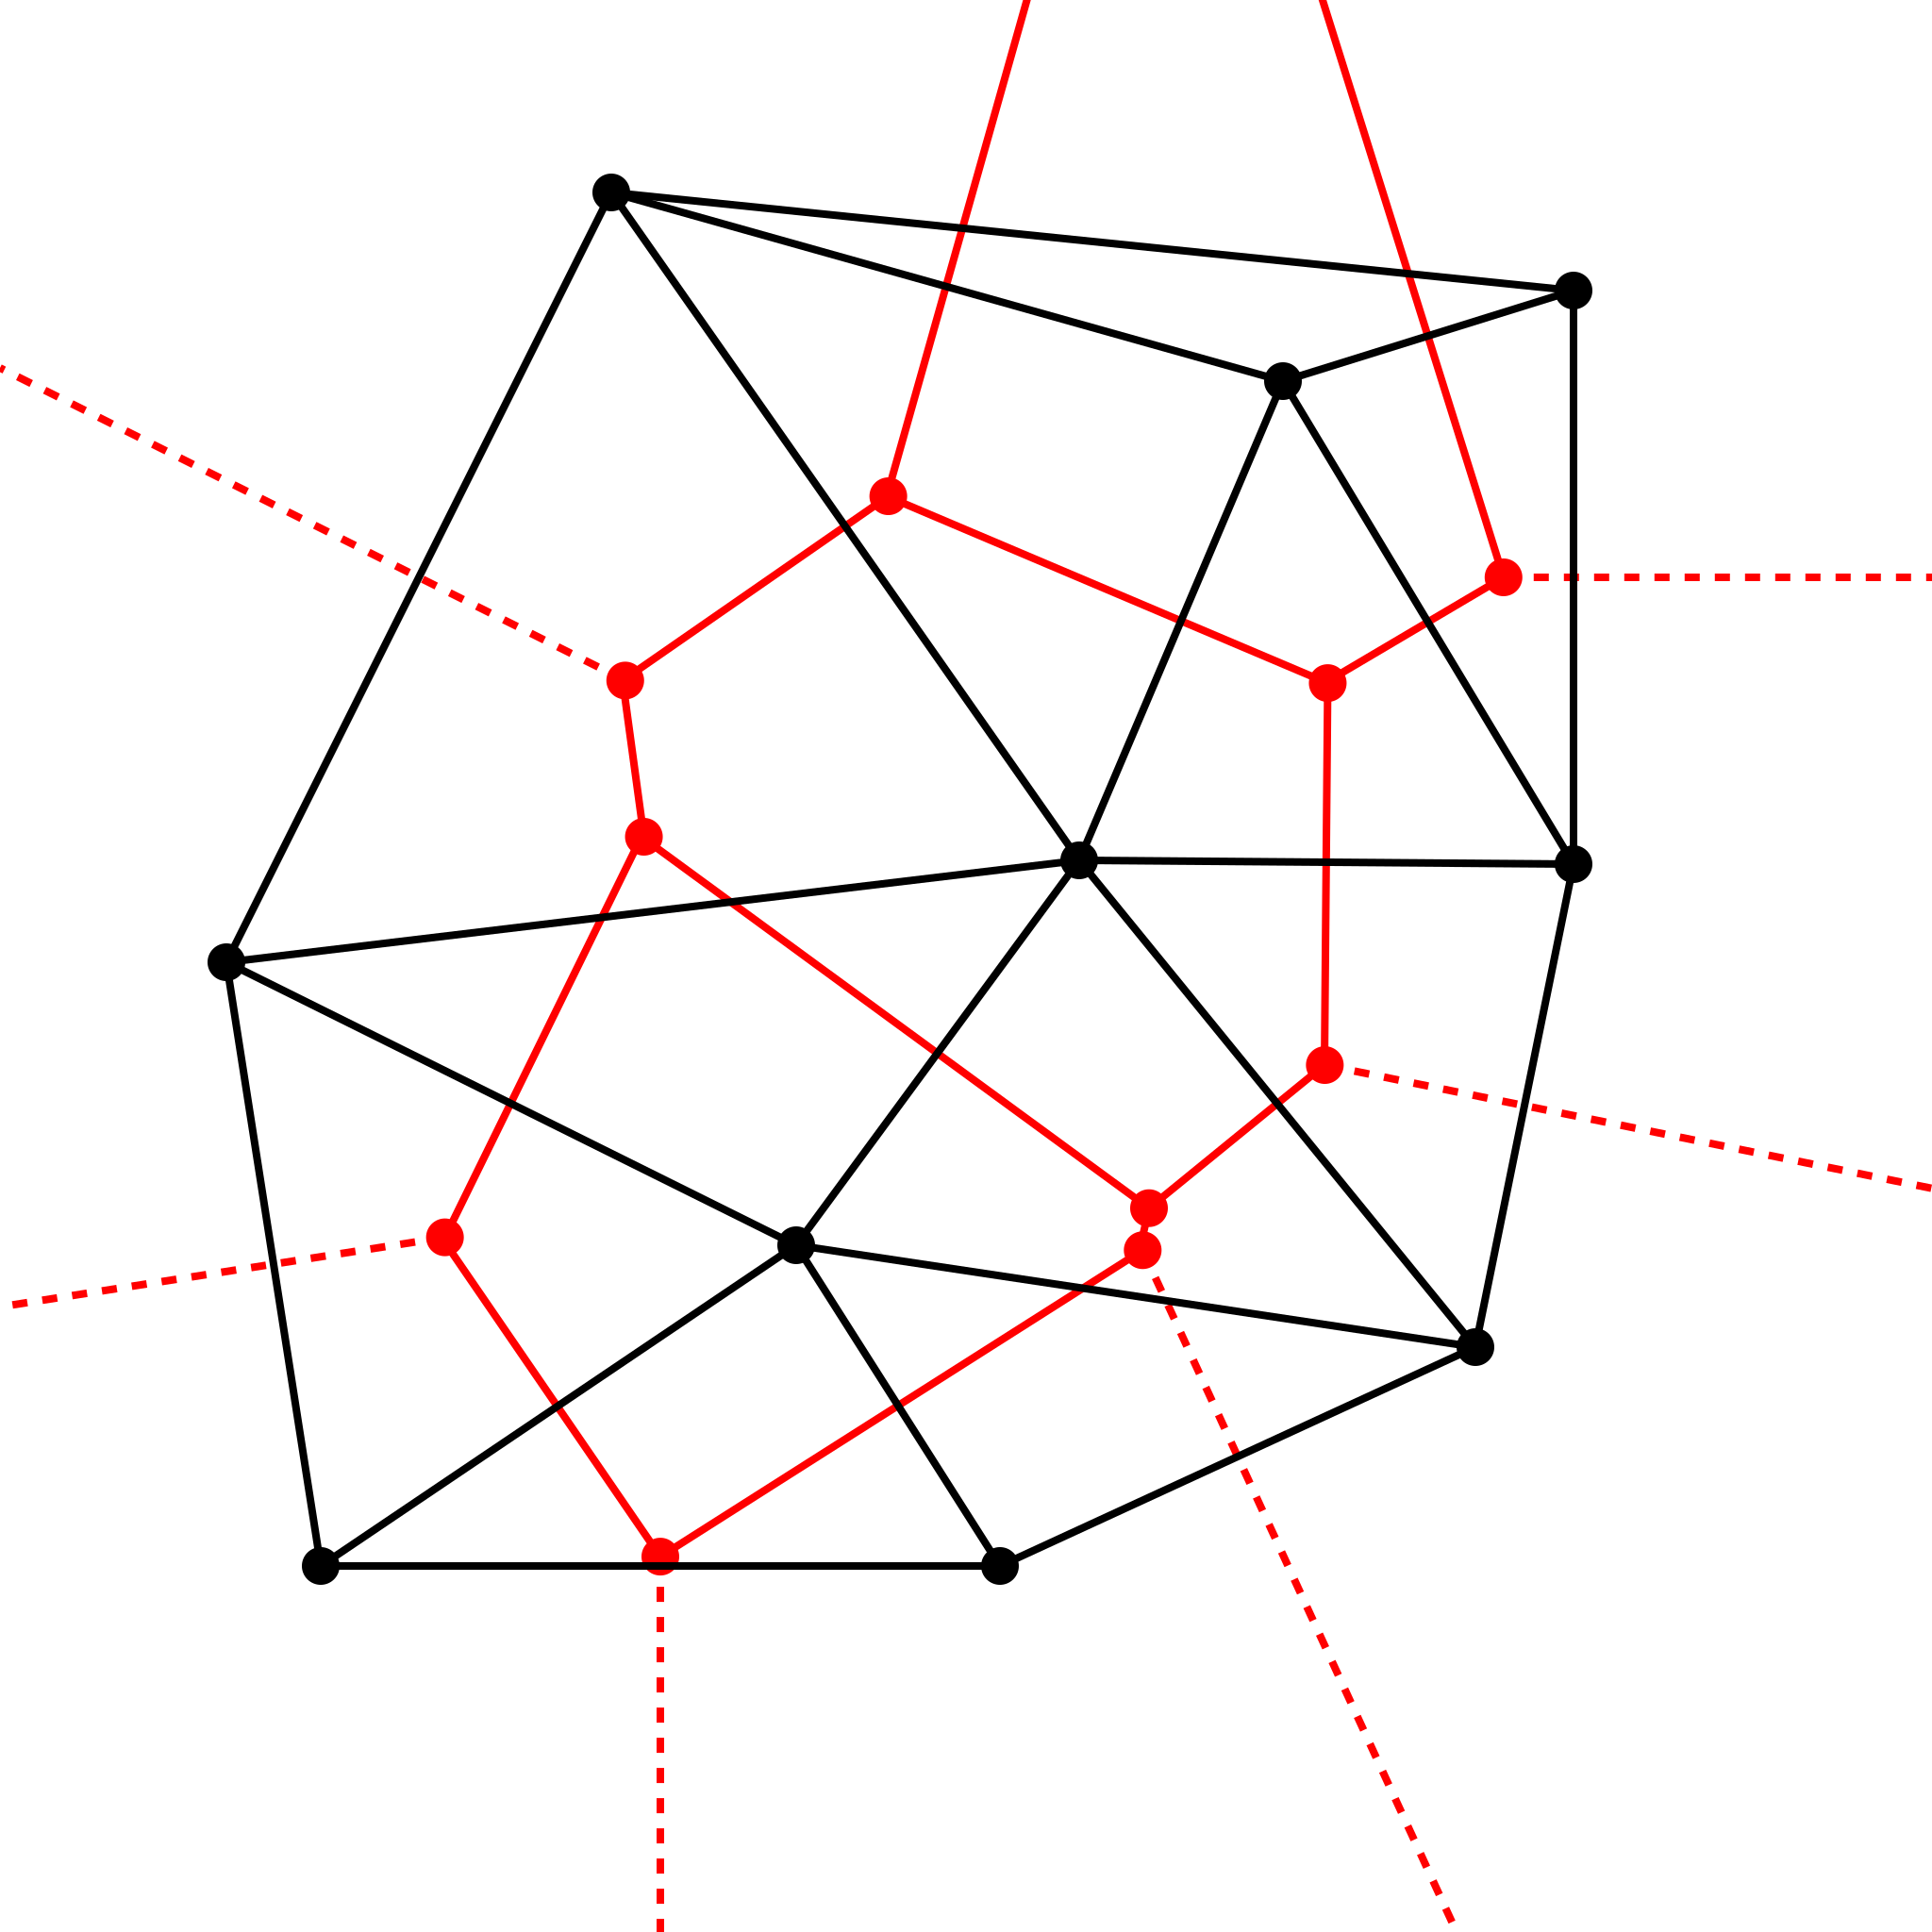
\includegraphics[width=1\linewidth]{delaunay-voronoi.png}
            \caption{Соединение центров описанных окружностей дает диаграмму Вороного (красного цвета).}
        \end{minipage}
    \end{center}
\end{figure}

\subsubsection*{Применение в решении}

Диаграмму Вороного можно использовать для решения поставленной задачи. Например:
\begin{enumerate}
    \item Временно удаляем искомую точку $x$ из множества $S$.
    \item Строим диаграмму Вороного для оставшихся точек.
    \item Ближайшим соседом точки $x$ будет точка $x'$, в область которой она попала.
\end{enumerate}

\newpage

\subsection{Алгоритмы}

Получается, для решения задачи нам необходимо построить либо диаграмму Вороного, либо триангуляцию Делоне. Рассмотрим алгоритмы для их нахождения.

\subsubsection*{Алгоритм слияния «Разделяй и властвуй» для построения триангуляции Делоне}

Данный алгоритм основан на стандартной для многих алгоритмов методике сведения сложной задачи к более простым, в которых решение очевидно. Сам алгоритм для $N>1$ состоит из 2 шагов:

\begin{enumerate}
    \item Разбиение исходного множества на более мелкие множества. Для этого мы проводим вертикальные или горизонтальные прямые в середине множества и уже относительно этих прямых разделяем точки на две части примерно по $N/2$. После для каждой группы точек рекурсивно запускаем процесс деления.
    \item Объединение оптимальных триангуляций. Сначала находятся две пары точек, отрезки которых образуют в совокупности с построенными триангуляциями выпуклую фигуру. Они соединяются отрезками, и один из полученных отрезков выбирается как начало для последующего обхода. Обход заключается в следующем: на этом отрезке мы как будто «надуваем пузырь» внутрь до первой точки, которую достигнет раздувающаяся окружность «пузыря». С найденной точкой соединяется та точка отрезка, которая не была с ней соединена. Полученный отрезок проверяется на пересечение с уже существующими отрезками триангуляции, и в случае пересечения они удаляются из триангуляции. После этого новый отрезок принимается за начало для нового «пузыря». Цикл повторяется до тех пор, пока начало не совпадёт со вторым отрезком выпуклой оболочки.
\end{enumerate}

Сложность разбиения множества $O(\log N)$, объединения —
$O(N)$ для каждого объединения, итоговая сложность алгоритма —
$O(N \log N)$.

\subsubsection*{Алгоритм Форчуна}

\textbf{Алгоритм Форчуна} — это алгоритм заметающей прямой для генерации диаграммы Вороного из набора точек на плоскости за время $O(n \log n)$ с использованием памяти $O(n)$.

\begin{figure}[H]
    \begin{center}
        \begin{minipage}[h]{0.3\linewidth}
            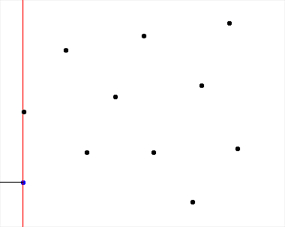
\includegraphics[width=1\linewidth]{fortunes-algo-00.jpg}
        \end{minipage}
        \hfill
        \begin{minipage}[h]{0.3\linewidth}
            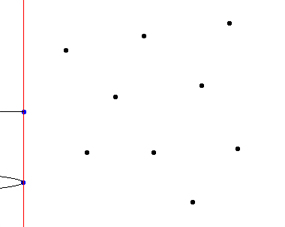
\includegraphics[width=1\linewidth]{fortunes-algo-01.jpg}
        \end{minipage}
        \hfill
        \begin{minipage}[h]{0.3\linewidth}
            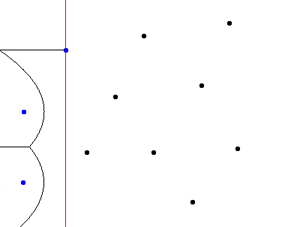
\includegraphics[width=1\linewidth]{fortunes-algo-02.jpg}
        \end{minipage}
    \end{center}
\end{figure}

\begin{figure}[H]
    \begin{center}
        \begin{minipage}[h]{0.3\linewidth}
            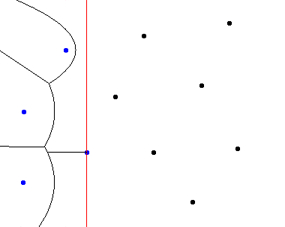
\includegraphics[width=1\linewidth]{fortunes-algo-03.jpg}
        \end{minipage}
        \hfill
        \begin{minipage}[h]{0.3\linewidth}
            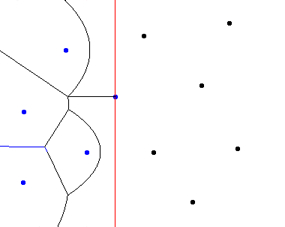
\includegraphics[width=1\linewidth]{fortunes-algo-04.jpg}
        \end{minipage}
        \hfill
        \begin{minipage}[h]{0.3\linewidth}
            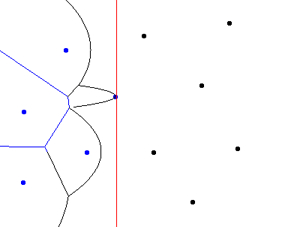
\includegraphics[width=1\linewidth]{fortunes-algo-05.jpg}
        \end{minipage}
    \end{center}
\end{figure}

\begin{figure}[H]
    \begin{center}
        \begin{minipage}[h]{0.3\linewidth}
            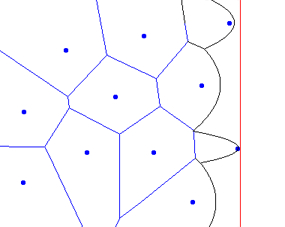
\includegraphics[width=1\linewidth]{fortunes-algo-19.jpg}
        \end{minipage}
        \hfill
        \begin{minipage}[h]{0.3\linewidth}
            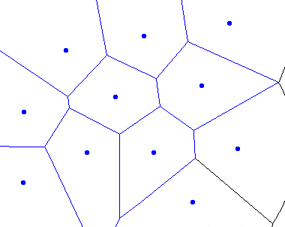
\includegraphics[width=1\linewidth]{fortunes-algo-20.jpg}
        \end{minipage}
        \hfill
        \begin{minipage}[h]{0.3\linewidth}
            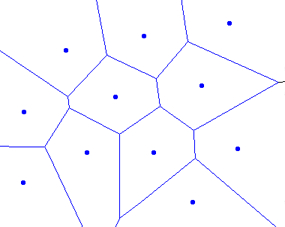
\includegraphics[width=1\linewidth]{fortunes-algo-21.jpg}
        \end{minipage}
    \end{center}
\end{figure}

Алгоритм поддерживает заметающую прямую и береговую линию, которые двигаются по плоскости в процессе работы алгоритма. Заметающая прямая — это прямая, которую мы по традиции можем считать вертикальной и движущейся слева направо. В любой момент работы алгоритма точки из набора слева от заметающей прямой будут включены в диаграмму Вороного, в то время как точки справа от заметающей прямой ещё не отработаны. Береговая линия не является прямой, а является сложной, состоящей из кусочков парабол, кусочно-заданной кривой слева от заметающей прямой. Она отделяет порцию плоскости, внутри которой диаграмма Вороного может быть известна, независимо от других точек справа от заметающей прямой. Для каждой точки слева от заметающей прямой можно определить параболу для точки, которая равноудалена как от этой точки, так и от заметающей прямой. Береговая линия — это граница объединений этих парабол. По мере движения прямой вершины береговой линии, в которых две параболы пересекаются, вычерчивают рёбра диаграммы Вороного. Береговая линия продвигается, сохраняя основание каждой параболы в точности на половину пути между начальным положением заметающей прямой и новой позицией заметающей прямой. Математически это значит, что каждая парабола образуется с помощью заметающей прямой как директрисы, а заданная точка из набора служит фокусом.

Алгоритм поддерживает структуру данных двоичного дерева, описывающего комбинаторную структуру береговой линии, и очередь с приоритетом, перечисляющую потенциальные события в будущем, которые могли бы изменить структуру береговой линии. Эти события включают добавление другой параболы в береговую линию (когда заметающая прямая проходит через другую входную точку) и удаление кривой из береговой линии (когда заметающая прямая становится касательной к окружности через некоторые три входных точки, параболы которых образуют последовательные сегменты береговой линии). Каждому такому событию может быть присвоен приоритет по x-координате заметающей прямой в точке, где событие произошло. Алгоритм состоит из последовательного удаления события из очереди с приоритетом, нахождения изменений событий в береговой линии и обновление структуры данных.

Так как имеется $O(N)$ событий для обработки (каждое ассоциировано с некоторым свойством диаграммы Вороного) и времени $O(\log N)$ для обработки события (которое состоит из постоянного числа поисков по двоичному дереву и операций очереди с приоритетом), общее время равно $O(N \log N)$.

